\chapter{Solution proposée}
\renewcommand{\leftmark}{\thechapter.~~Solution}
Dans le chapitre précédent, les différentes solutions existantes pour faire
du CCMP ont été analysées. La solution jugée la plus efficace
est Remote Clip, celle-ci proposant une architecture P2P adéquate et un
niveau de sécurité correct. Pour ces raisons, certaines idées mises en avant
par Remote Clip seront réutilisées. De même des messages seront envoyés en
broadcast afin d'auto-configurer le réseau comme fait dans The Network
Clipboard.

\section{Principes d'une architecture P2P}\label{sec:p2p}
Avant de décrire l'architecture qui sera utilisée, il est préférable
de rappeler quels sont les principes de base d'une architecture P2P.
Habituellement, une architecture client-serveur est utilisée lorsqu'il
faut fournir un service à un ensemble de machines connectées en réseau,
c'est-à-dire que chaque client va se connecter à un (ou parfois plusieurs)
serveur central qui s'occupera de fournir le service désiré. Par opposition à
ce mode de fonctionnement centralisé, un réseau organisé en pair-à-pair
permet de se passer de serveur central, chaque client jouant à la fois le rôle
de client et de serveur. La figure \ref{fig:p2p} illustre la différence
de topologie réseau existante entre ces deux types d'architectures réseau.
De manière plus précise les systèmes P2P sont définis dans \cite{AS04} comme
étant:
\begin{quote}
  des systèmes distribués constitués de noeuds interconnectés, capables de
  s'auto-organiser dans des topologies de réseaux avec comme but le partage
  de ressources, telles que le contenu, les cycles CPU, le stockage,
  la bande passante tout en ayant la capacité de s'adapter aux erreurs et
  de s'accommoder de populations de noeuds transitoires; tout en maintenant
  une connectivité et des performances acceptables sans requérir
  l'intermédiaire ou le support d'un serveur ou d'une autorité
  centralisée globalement.
\end{quote}

Les difficultés potentielles à mettre en avant dans ce genre de systèmes
sont la gestion des va-et-vient de clients et la tolérance aux erreurs
sans l'aide de serveur central, et tout en minimisant la charge sur le réseau,
due à cette gestion. Il faut cependant noter que l'importance de la tolérance
aux erreurs est tout de même assez minime dans le contexte du copier/coller.
Les données stockées sont en général destinées à être utilisées à court terme
et non pas à être stockées de manière persistante. De même le nombre de pairs
est normalement peu élevé, et donc le nombre de va-et-vient n'est pas aussi
important que sur des systèmes à grande échelle.

Une remarque supplémentaire à faire est qu'une différence est souvent faite
entre réseaux P2P structurés et non structurés \cite{AS04, Lua05asurvey}.
Les premiers ont une topologie contrôlée de manière précise permettant
de placer chaque donnée à un endroit précis et d'effectuer des recherches
efficaces. Le réseau ici étant censé être de taille relativement petite
et le contenu changeant très rapidement, il n'est pas nécessaire de structurer
le réseau. En effet, le fait de structurer le réseau, en utilisant par exemple
une table de hashage distribuée, a comme intérêt d'avoir une complexité
algorithmique sous-linéaire en fonction du nombre de pairs présent dans
le réseau. Ici la taille du réseau étant fortement réduite, cette
complexité a peu d'impact sur les performances du logiciel. Le fait de ne
pas utiliser une table de hashage distribuée permet donc d'avoir un protocole
plus simple sans perte de performances.

\begin{figure}[!h]
  \centering
  % \input{fig_p2p.tex}
  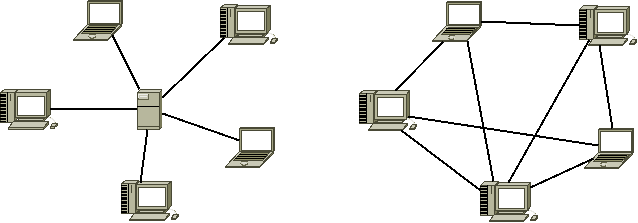
\includegraphics[width=\textwidth]{fig_p2p}
  \caption{Exemple de différence entre une topologie client-serveur et P2P}
  \label{fig:p2p}
\end{figure}

\section{Architecture logicielle}
Afin de suivre le principe \emph{KISS} (Keep It Simple Stupid, \emph{cf.}
Annexe \ref{ann:kiss}) et la philosophie Unix, le projet sera divisé en
plusieurs programmes, chacun d'entre eux s'occupant d'une tâche particulière.
Une autre raison justifiant une telle conception est le fait qu'elle introduit
la possibilité de développer le projet de manière incrémentale, en se
concentrant d'abord sur l'aspect réseau et ensuite sur l'implémentation
propre à un environnement particulier.

\subsection{Client P2P}
Premièrement un logiciel s'occupant uniquement de la gestion du presse-papier
sur le réseau est nécessaire. Celui-ci a comme rôle de se connecter aux
autres pairs et de s'organiser avec ceux-ci quand cela est nécessaire.
Sa seule fonctionnalité est en fait de gérer la partie réseau du système,
toute interaction locale (\emph{i.e.} avec l'utilisateur) se fait par
l'intermédiaire d'autres logiciels qui seront définis par la suite.

Il faut définir de manière plus précise comment l'ensemble des clients P2P
vont s'organiser afin de s'informer pour savoir quel client \emph{détient} le
presse-papier, comment un pair entre dans le réseau et comment détecter
qu'un pair a quitté celui-ci (volontairement ou pas). Des exemples
de fonctionnement de cette architecture et du protocole qui seront mis en
oeuvre sont montrés dans les figures \ref{fig:join} et \ref{fig:copypaste}.

\subsubsection*{Gestion du presse-papier en P2P}
Il y a principalement deux possibilités pour gérer le presse-papier
sur le réseau. Lorsqu'un copier est effectué en local, le client P2P
doit prévenir les autres pairs qu'il détient le presse-papier.
La première option est d'envoyer en même temps la donnée copiée à tous les
pairs. La deuxième est de n'envoyer cette donnée que lorsque qu'un coller
est effectué chez un pair, celui-ci peut alors demander la donnée au pair
détenant le presse-papier.\\\\
La première manière de faire a les avantages et inconvénients suivants:
\begin{itemize}
\item Avantages:
  \begin{itemize}
  \item Possibilité de garder une copie du presse-papier sur chaque pair.
  \item Tolérance aux erreurs dans le cas où le pair détenant le presse-papier
    aurait quitté le réseau.
  \item Absence de communications réseaux en cas de multiples coller.
  \end{itemize}
\item Inconvénients:
  \begin{itemize}
  \item Consommation de bande passante accrue dans le cas où des copiers
    sont effectués fréquemment car il faudra envoyer la même donnée à chacun
    des pairs qui ne feront peut être pas forcément de coller. De plus la
    consommation de bande passante dépend du nombre de pair présent sur le
    réseau.
  \end{itemize}
\end{itemize}
La seconde a les avantages et inconvénients suivants:
\begin{itemize}
\item Avantages:
  \begin{itemize}
  \item Il n'est pas nécessaire de notifier l'ensemble des pairs à chaque
    copier: si un pair effectue plusieurs copies d'affilée, il ne faudrait
    notifier le réseau qu'une seule fois et sans envoyer la moindre donnée.
  \item En général le coller ne sera effectué que par un seul pair,
    il n'a donc qu'à demander lui même au pair détenant le presse-papier
    de la lui envoyer.
  \end{itemize}
\item Inconvénients:
  \begin{itemize}
  \item Impossibilité de récupérer le presse-papier d'un pair ayant quitté
    le réseau.
  \item Si plusieurs collers ont lieu les uns à la suite des autres, il faudra
    demander plusieurs fois la même donnée au pair détenant le presse-papier.\\
  \end{itemize}
\end{itemize}

Il est donc nécessaire de faire un choix entre une de ces options
et c'est la seconde qui est choisie. C'est ainsi que fonctionne non seulement
Remote Clip, mais aussi X Window\cite{nye1992xlib} à la différence
que c'est une architecture client-serveur qui est utilisée. En effet, X Window
est un serveur qui considère chaque fenêtre comme un client. Lorsque
l'utilisateur copie un élément de cette fenêtre, elle notifie le serveur X
qu'elle détient le presse-papier. Ensuite lorsque l'utilisateur
veut coller le contenu du presse-papier, la fenêtre dans laquelle est
effectuée le coller doit demander au serveur X quel client détient le
presse-papier et ensuite s'adresser à celui-ci pour l'obtenir. L'application
devant viser en priorité le monde Unix, c'est ce principe qui est adapté à
une architecture sans serveur. Il faut aussi noter que sous X, il n'est pas
possible de savoir si le presse-papier a changé: si deux copies sont
effectuées au sein de la même application, il n'y a qu'une seule notification
qui est faite auprès des autres fenêtres, il faudrait donc constamment
vérifier que celui-ci a changé ou pas afin de le synchroniser sur le
réseau.

\subsubsection*{Rejoindre le réseau}
Outre un moyen d'authentification, il est nécessaire de définir comment
un pair peut rejoindre le réseau afin de partager son presse-papier.
Une première solution consiste en la connaissance, pour un pair voulant
rejoindre le réseau, de connaître l'IP et l'identifiant d'au moins un autre
pair déjà présent dans le réseau et connaissant les autres pairs présents
dans ce réseau. Il suffit alors de contacter cet autre pair et de synchroniser
la  liste des pairs de l'ensemble du réseau. Une autre solution envisageable
est d'utiliser un mécanisme de broadcast permettant de flooder le réseau pour
rechercher les pairs désirant rejoindre le réseau. Cette solution sera celle
utilisée, celle-ci permettant de minimiser le nombres de paramètres que devra
configurer l'utilisateur.

Pour cela, il faut que chaque pair envoie à interval régulier un message
en broadcast, sur le réseau local, permettant d'identifier le groupe de pairs
auquel il appartient ou veut appartenir. Tout pair appartenant au groupe et
recevant le message doit alors contacter le pair ayant envoyé le message en
ouvrant une connexion TCP sécurisée. Il faut cependant faire attention à un
problème: le nombre de connexions TCP ouvertes peut devenir une charge
importante pour le réseau. En effet pour un groupe de $n$ pair, $n-1$
connexions sera ouverte pour chaque pair. Le nombre de connexions serait donc
en $(O(n^2)$. Cependant le réseau P2P étant limité à quelques pairs dans le
cas du CCMP, ceci n'est pas handicapant.

\subsubsection*{Quitter le réseau}
Lorsqu'un pair quitte le réseau, il doit notifier l'ensemble des autres
pairs de son départ. Une fois ceci fait, il peut fermer chaque connexion
ouverte avec chacun des pairs. En revanche il se peut qu'un pair quitte
le réseau sans pouvoir notifier les pairs de son départ, \emph{e.g.}
à cause d'une déconnexion du lien physique. Pour cela un mécanisme
de \emph{keep alive} doit être utilisé. Il faut que chaque pair envoie
de manière régulière un message sur chaque connexion ouverte, même en cas
d'inactivité de la part de l'utilisateur. Lorsqu'un pair n'envoie plus
de messages keep alive pendant un certain laps de temps, il faut que les
autres pairs ferment la connexion TCP avec ce pair et le considèrent comme
ayant quitté le réseau. Si la connexion physique est rétablie, le pair
\emph{disparu} peut alors rejoindre à nouveau le réseau grâce au mécanisme
de broadcast.

\subsection{Client local}
Le client P2P est le \emph{front-end} avec le réseau, il est chargé
de communiquer avec les pairs du réseau afin de les découvrir et savoir
lequel détient le presse-papier. Le front-end avec l'utilisateur
est en revanche le client local. Celui-ci tourne sur le même ordinateur
que le client P2P, se charge de notifier le client P2P lorsque
l'utilisateur copie quelque chose et le notifie lorsqu'il désire
accéder au presse-papier. Le client P2P notifie le client local
lorsqu'un pair du réseau détient le presse-papier c'est-à-dire lorsque ce
pair effectue un copir.
Un exemple d'interaction entre clients locaux et clients P2P utilisant
le protocole qui sera mis en oeuvre est montré sur la figure \ref{fig:local}.

Cependant, contrairement au client P2P, il peut y avoir plusieurs clients
locaux tournant sur le même ordinateur. Chacun d'entre eux étant destiné
à un environnement précis. Dans ce projet, seront développés deux types
de clients différents:
\begin{itemize}
\item Un client tournant en tâche de fond (comme \emph{daemon}) et
  synchronisant le contenu du presse-papier de X Window.
\item Un client gérant le copier/coller dans un terminal, composé de trois
  logiciels:
  \begin{itemize}
  \item Un daemon gérant le presse-papier, cette fonctionnalité n'étant en
    général pas implémentée dans un shell, seuls les émulateurs de terminaux
    peuvent communiquer avec celui de X Window.
  \item Une commande permettant de copier une donnée à partir de l'entrée
    standard du shell.
  \item Une commande permettant de coller une donnée sur la sortie standard
    du shell.
  \end{itemize}
\end{itemize}
Il est à noter que dans le cas du premier client, le rôle des deux commandes
est en fait joué par les clients X Window \emph{i.e.} les fenêtres ouvertes
et réalisant le copier/coller.

\section{Protocoles}
Deux protocoles sont à définir afin de faire fonctionner l'application
correctement. Le premier est celui utilisé sur le réseau par les clients
P2P afin de communiquer entre eux. Le second est utilisé entre le client
P2P et les clients locaux afin de se notifier mutuellement de changements
dans le presse papier. De même ils doivent tous les deux prendre en compte
l'aspect sécurité, en proposant un moyen d'identification.
Ces deux protocoles seront appelés respectivement protocole P2P et protocole
local.

Les protocoles sont caractérisés par un ensemble de types de messages.
Ceux-ci sont décrits en utilisant la syntaxe suivant:
\begin{verbatim}
MSG <SP> <VAR1> <SP> <VAR2> ... <SP> <VARN> <LF>
\end{verbatim}
MSG définit le type du message. Celui-ci contient $N$ variables
<VAR1>, <VAR2>, $\ldots$, <VARN>. Chacune est séparée par un espace (<SP>)
et le message se termine par un passage à ligne (<LF>). Chaque variable est
ensuite décrite et le type de messages pouvant être reçu comme réponse est
décrit.

\subsection{Protocole P2P}
\subsubsection*{AUTH}
Afin de s'authentifier lors de l'ouverture d'une connexion TCP/TLS,
un identifiant est choisi pour le pair et un mot de passe est défini dans la
configuration du client.
Lorsqu'un pair veut contacter pour la première fois un pair, il doit
s'authentifier auprès de celui-ci. Pour cela il envoie un message
d'authentification:
\begin{verbatim}
AUTH <SP> <NAME> <SP> <PSWD> <LF>
\end{verbatim}
\begin{description}
\item[Variable NAME:] identifiant de l'hôte à joindre.
\item[Variable PSWD:] mot de passe.
\item[Réponse:] si le mot de passe est correct \emph{i.e.} est le même
  utilisé par les deux pairs, le pair contacté peut accepter la connexion
  et répondre par un message de type OK, sinon il répond par un message de type
  KO avec un code d'erreur 1.
\end{description}

\subsubsection*{OK}
Ce type de message permet de confirmer la plupart des opérations:
\begin{verbatim}
OK <LF>
\end{verbatim}

\subsubsection*{KO}
Ce type de message permet de signaler un refus ou une erreur:
\begin{verbatim}
KO <SP> <ERRNO> <LF>
\end{verbatim}
\begin{description}
\item[Variable ERRNO: ] code d'erreur pouvant être:
  \begin{description}
  \item[0] erreur non définie/générique.
  \item[1] échec d'authentification.
  \item[2] pair non valide.
  \end{description}
\end{description}

\subsubsection*{JOIN}
Un message de type JOIN permet de rejoindre le réseau:
\begin{verbatim}
JOIN <SP> <TYPE> <SP> <NAME1> <SP> <NAME2> <LF>
\end{verbatim}
\begin{description}
\item[Variable NAME1:] identifiant du pair.
\item[Variable NAME2:] identifiant du pair contacté.
\item[Variable TYPE:]
  \begin{description}
  \item[0] signifie que le pair n'a pas encore obtenu la liste des pairs
  \item[1] signifie que le pair a déjà la liste des pairs
  \end{description}
\item[Réponse:] si l'identifiant du pair contacté n'est pas le bon, la
  réponse est un message KO avec un code d'erreur 2, si celui-ci est bon la
  réponse est un message de type LIST si le pair a besoin de la liste des
  pairs, sinon un message de type OK.
\end{description}

\subsubsection*{LIST}
Un message de type LIST annonce une liste de messages de type PEER:
\begin{verbatim}
LIST <SP> <N> <LF>
\end{verbatim}
\begin{description}
\item[Variable N:] nombre de messages PEER qui suivent.
\end{description}

\subsubsection*{PEER}
Un message de type PEER décrit ce qui identifie un pair:
\begin{verbatim}
PEER <SP> <NAME> <SP> <IP> <SP> <PORT> <LF>
\end{verbatim}
\begin{description}
\item[Variable NAME:] identifiant du pair permettant d'effectuer un JOIN.
\item[Variable IP:] adresse IP permettant de joindre le pair.
\item[Variable PORT:] port sur lequel le pair écoute.
\end{description}

\subsection*{LEAVE}
Un message de type LEAVE doit être envoyé pour quitter le réseau et ne
nécessite aucune réponse:
\begin{verbatim}
LEAVE <LF>
\end{verbatim}

\subsubsection*{COPY}
Un message de type COPY est envoyé lorsque le pair détient le presse-papier:
\begin{verbatim}
COPY <LF>
\end{verbatim}

\subsubsection*{PASTE}
Un message de type PASTE est envoyé lorsqu'un pair doit obtenir le
presse-papier:
\begin{verbatim}
PASTE <LF>
\end{verbatim}
\begin{description}
\item[Réponse:] Un message de type DATA. Si le pair ne possède pas le
  presse-papier un message de type PEER doit être envoyé avec les informations
  du pair détenant le presse-papier.
\end{description}

\subsubsection*{DATA}
Un message de type DATA permet d'envoyer le contenu du presse-papier:
\begin{verbatim}
DATA <SP> <TYPE> <SP> <LENGTH> <SP> <CONTENT> <LF>
\end{verbatim}
\begin{description}
\item[Variable TYPE:] cette variable permet de préciser le type
  de donnée et ainsi d'étendre facilement le protocole afin de supporter
  d'autres types de données. Dans ce cas il faudra préciser comment ce type
  de données est encodé.
  \begin{description}
  \item[0] type non défini/inconnu.
  \item[1] texte.
  \end{description}
\item[Variable LENGTH:] longueur de la donnée.
\item[Variable CONTENT:] contenu de la donnée dont la longueur
  doit vérifier la variable LENGTH.
\end{description}

\begin{figure}[!h]
  \centering
  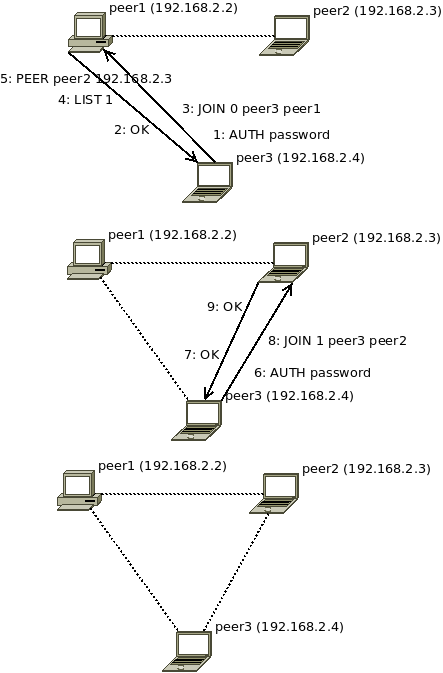
\includegraphics[width=0.9\textwidth]{fig_join}
  \caption{Le pair 3 qui rejoint un réseau. Les lignes en pointillés
    représentent les pairs qui se connaissent mutuellement \emph{i.e.} qui ont
    une connexion TCP/TLS ouverte, et les flèches les communications réseaux
    entre deux pairs. Les messages envoyés sont numérotés afin de suivre
    l'ordre dans lequel ils sont envoyés.}
  \label{fig:join}
\end{figure}

\begin{figure}[!h]
  \centering
  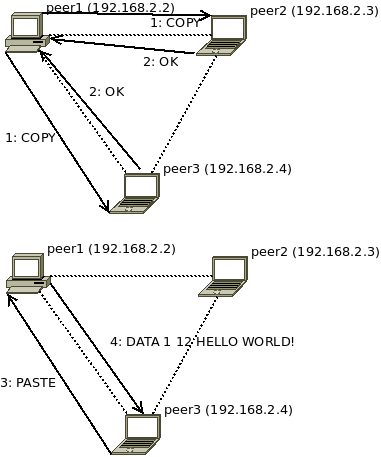
\includegraphics[width=0.9\textwidth]{fig_copypaste}
  \caption{Exemple de copier/coller: le pair 1 copie le texte HELLO WORLD!
    et l'envoie au pair 3 qui fait un coller. Les lignes en pointillés
    représentent les pairs qui se connaissent mutuellement \emph{i.e.} qui ont
    une connexion TCP/TLS ouverte, et les flèches les communications réseaux
    entre deux pairs. Les messages envoyés sont numérotés afin de suivre
    l'ordre dans lequel ils sont envoyés.}
  \label{fig:copypaste}
\end{figure}

\subsection{Protocole local}
Le protocole local utilise un sous-ensemble des messages du protocole P2P,
celui-ci ayant seulement besoin de notifications de copier/coller et de
s'authentifier.
Les messages utilisés seront ceux de type AUTH, OK, KO, COPY, PASTE et DATA.
Les messages de type AUTH, OK et KO sont toujours utilisés pour
l'authentification.

La sémantique des messages de type COPY change légèrement: le client
local envoie un tel message lorsque l'utilisateur copie une donnée dans le
presse-papier et le client P2P envoie un COPY au client local lorsque
c'est un autre pair (ou un autre client local) qui détient le presse-papier.

Les messages de type PASTE sont quant à eux envoyés lorsque le client local
désire faire un coller et qu'il ne détient pas le presse-papier ou bien
lorsqu'un autre pair désire obtenir le contenu du presse-papier détenu par le
client local. Les messages de type DATA ont toujours la même sémantique:
servir de réponse à un message de type PASTE.

\begin{figure}[!h]
  \centering
  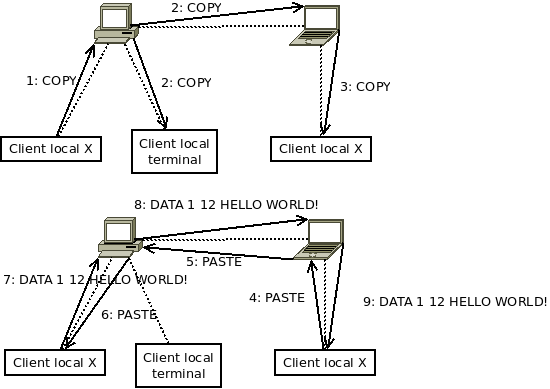
\includegraphics[width=0.9\textwidth]{fig_local}
  \caption{Exemple de copier/coller avec clients locaux. Les lignes en
    pointillés représentent les pairs qui se connaissent mutuellement
    \emph{i.e.} qui ont une connexion TCP/TLS ouverte, et les flèches les
    communications réseaux entre deux pairs. Les messages envoyés sont
    numérotés afin de suivre l'ordre dans lequel ils sont envoyés.}
  \label{fig:local}
\end{figure}

\begin{figure}[!h]
  \centering
  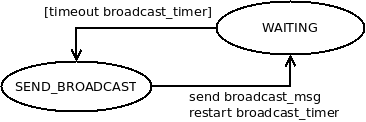
\includegraphics[width=0.9\textwidth]{p2pclient_broadcast}
  \caption{P2P Client Broadcast}
  \label{fig:p2pclient_broadcast}
\end{figure}

\begin{figure}[!h]
  \centering
  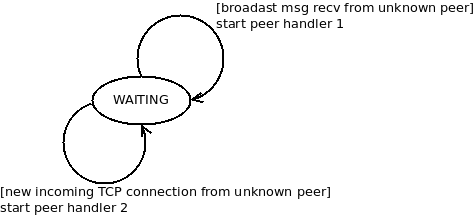
\includegraphics[width=0.9\textwidth]{p2pclient_connections}
  \caption{P2P Client Connections}
  \label{fig:p2pclient_connections}
\end{figure}

\begin{figure}[!h]
  \centering
  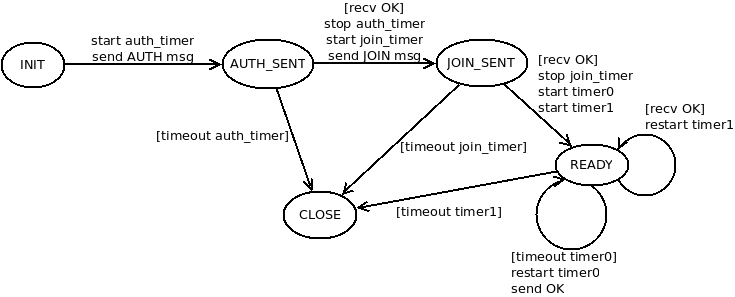
\includegraphics[width=0.9\textwidth]{p2pclient_peerhandler1}
  \caption{P2P Client Peer Handler 1}
  \label{fig:p2pclient_peerhandler1}
\end{figure}

\begin{figure}[!h]
  \centering
  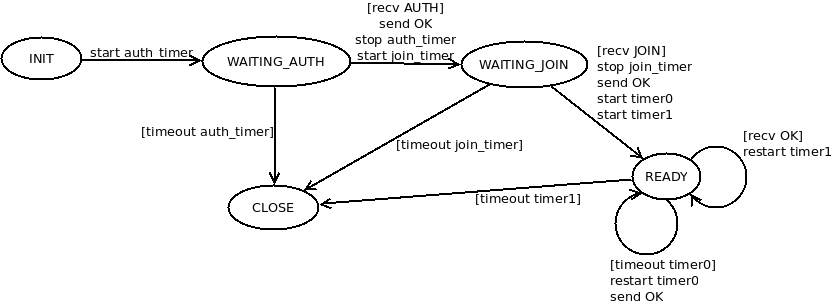
\includegraphics[width=0.9\textwidth]{p2pclient_peerhandler2}
  \caption{P2P Client Peer Handler 2}
  \label{fig:p2pclient_peerhandler2}
\end{figure}
